\documentclass[twoside]{article}

\usepackage{graphicx} % Required for inserting images
\usepackage{amsmath}
\usepackage{amsfonts}
\usepackage{amssymb}
\usepackage{siunitx}
\usepackage{layout}
\usepackage{titlesec}
\usepackage{etoolbox}
\usepackage{cancel}
\usepackage{xcolor}


\usepackage{geometry}
\usepackage[skip=\bigskipamount, indent]{parskip} % bigskip between paragraphs
\usepackage{lipsum}
\usepackage[most]{tcolorbox}
\usepackage{pgfplots}
\usepackage{tikz}
\usetikzlibrary{arrows}
\usepackage{calc}
\usepackage{hyperref}
\usepackage{fourier-orns}
\usepackage{fontawesome5}
\usepackage{fancyhdr}


\geometry{top = 1.0in, bottom = 1.0in, left = 0.9in, right = 0.9in} % Set page margins

\definecolor{RoyalBlue}{HTML}{16348C} % Section title colour
\definecolor{DeepPurple}{HTML}{440150} % Subsection title colour
\definecolor{DeepGreen}{HTML}{0B6623} % Subsubsection title colour
\definecolor{DeepLavendar}{HTML}{7373E3} % Question box boundary colour
\definecolor{Lavendar}{HTML}{E6E6FA} % Question box colour
\definecolor{DeepTeaGreen}{HTML}{62C92F} % Answer box boundary colour
\definecolor{TeaGreen}{HTML}{D1F5BF} % Answer box colour
\definecolor{DeepBubbleGumBlue}{HTML}{57CEEE} % Remarks box boundary colour
\definecolor{BubbleGumBlue}{HTML}{CDF9FA} % Remarks box colour
\definecolor{Cream}{HTML}{FDFCC3} % Derivation box colour
\definecolor{DeepCream}{HTML}{FBF65E} % Derivation box boundary colour
\definecolor{Almond}{HTML}{F4E7DB} % Example box colour
\definecolor{DeepAlmond}{HTML}{E0BE9C} % Example box boundary colour
\definecolor{MidnightBlue}{HTML}{191970} % Hyperlink colour
\definecolor{CobaltBlue}{HTML}{0047AB} % Reference colour



\newlength\titleindent
\setlength\titleindent{3em} % Title indentations
\setlength\parindent{0pt} % No indent for all paragraphs

\titleformat{\section}{\normalfont\Large\bfseries\color{RoyalBlue}}{\llap{\parbox{\titleindent}{\thesection\hfill}}}{0em}{}
\titleformat{\subsection}{\normalfont\normalsize\bfseries\color{DeepPurple}}{\llap{\parbox{\titleindent}{\thesubsection\hfill}}}{0em}{}
\titleformat{\subsubsection}{\normalfont\normalsize\bfseries\color{DeepGreen}}{\llap{\parbox{\titleindent}{\thesubsubsection\hfill}}}{0em}{}

\pgfplotsset{compat = 1.18}

\hypersetup{
	colorlinks = true,
	urlcolor = MidnightBlue,
	linkcolor = CobaltBlue,
}

% Define the volume symbol
\makeatletter
\DeclareRobustCommand{\vol}{\text{\volumedash}V}
\newcommand{\volumedash}{%
	\makebox[0pt][l]{%
		\ooalign{\hfil\hphantom{$\m@th V$}\hfil\cr\kern0.16em\rotatebox{27.5}{\textbf{--}}\hfil\cr}%
	}%
}
\makeatother


% Define definition box
\newtcolorbox{definitionbox}{enhanced, parbox = false, boxrule = 0mm, boxsep = 0mm,
							 arc = 0mm, outer arc = 0mm,
							 left = 4mm, right = 3mm, top = 7pt, bottom = 7pt,
							 toptitle = 1mm, bottomtitle = 1mm, oversize,
							 borderline west = {5pt}{0pt}{DeepLavendar}, colback = Lavendar}
\newcommand{\definition}[1]{\begin{definitionbox} \textcolor{red}{{\scriptsize\faStar} \textbf{Definition}} \newline #1 \end{definitionbox}}

% Define answer box
\newtcolorbox{answerbox}{enhanced, parbox = false, boxrule = 0mm, boxsep = 0mm,
	arc = 0mm, outer arc = 0mm,
	left = 4mm, right = 3mm, top = 7pt, bottom = 7pt,
	toptitle = 1mm, bottomtitle = 1mm, oversize,
	borderline west = {5pt}{0pt}{DeepTeaGreen}, colback = TeaGreen}
\newcommand{\answer}[1]{\begin{answerbox} \emoji{melon} \textbf{Answer} \newline #1 \end{answerbox}}

% Define remarks box
\newtcolorbox{remarksbox}{enhanced, parbox = false, boxrule = 0mm, boxsep = 0mm,
	arc = 0mm, outer arc = 0mm,
	left = 4mm, right = 3mm, top = 7pt, bottom = 7pt,
	toptitle = 1mm, bottomtitle = 1mm, oversize,
	borderline west = {5pt}{0pt}{DeepBubbleGumBlue}, colback = BubbleGumBlue}
\newcommand{\remarks}[1]{\begin{remarksbox} \emoji{blueberries} \textbf{Remarks} \newline #1 \end{remarksbox}}

% Define derivation box
\newtcolorbox{derivationbox}{enhanced, parbox = false, boxrule = 0mm, boxsep = 0mm,
	arc = 0mm, outer arc = 0mm,
	left = 4mm, right = 3mm, top = 7pt, bottom = 7pt,
	toptitle = 1mm, bottomtitle = 1mm, oversize,
	borderline west = {5pt}{0pt}{DeepCream}, colback = Cream}
\newcommand{\derivation}[1]{\begin{derivationbox} \emoji{pineapple} \textbf{Equation Derivation} \newline #1 \end{derivationbox}}

% Define derivation box
\newtcolorbox{examplebox}{enhanced, parbox = false, boxrule = 0mm, boxsep = 0mm,
	arc = 0mm, outer arc = 0mm,
	left = 4mm, right = 3mm, top = 7pt, bottom = 7pt,
	toptitle = 1mm, bottomtitle = 1mm, oversize,
	borderline west = {5pt}{0pt}{DeepAlmond}, colback = Almond}
\newcommand{\example}[1]{\begin{examplebox} \emoji{croissant} \textbf{Example} \newline #1 \end{examplebox}}

% Define blue text
\newcommand{\highlightbluetext}[1]{\textcolor[HTML]{09ACA6}{\textbf{#1}}}

% Define green text
\newcommand{\highlightgreentext}[1]{\textcolor[HTML]{62C92F}{\textbf{#1}}}

% Numbers with circle
\newcommand*\circled[1]{\tikz[baseline=(char.base)]{\node[shape=circle,draw,inner sep=2pt] (char) {#1};}}

\numberwithin{equation}{section}

\usetikzlibrary{arrows.meta, positioning}

\begin{document}
	\begin{titlepage}
		\centering
		\scshape
		\vspace*{\baselineskip}
		
		\rule{\textwidth}{1.6pt}\vspace{-\baselineskip}\vspace{2pt} % Thick horizontal rule
		\rule{\textwidth}{0.4pt} % Thin horizontal rule
		
		\vspace{0.5\baselineskip}
		
		{\LARGE \textbf{COMP4211 \\ Machine Learning} \\
			
			\vspace{0.75\baselineskip}
			\Large Notes}
		
		\vspace{0.5\baselineskip}
		
		\rule{\textwidth}{0.4pt}\vspace{-\baselineskip}\vspace{3.2pt} % Thin horizontal rule
		\rule{\textwidth}{1.6pt} % Thick horizontal rule
		
		\vspace{1.5\baselineskip}
		
		{\large Insturctor: Dit Yan, Yeung \\
			\vspace{0.5\baselineskip} Fall 2025}
		
		\vspace{\baselineskip}
		
		{\Large Edited by \\
			\vspace{0.5\baselineskip}
			\Large ThunderDora \\

			\vspace{10pt}
			\large \textit{The Hong Kong University of Science and Technology}}
		
		\vspace{10\baselineskip}
		
		\textit{Last Edited: \textbf{\today}}
		
	\end{titlepage}
	
	\newpage
	
	% Configure the headers and footers
	\pagestyle{fancy}
	\fancyhf{}
	\renewcommand{\headrulewidth}{0pt}
	\fancyhead[C]{\large \textbf{COMP4211 - Machine Learning}}
	
	\fancyfoot{}

	\fancyfoot[RO, LE]{\thepage}
	
	\setcounter{page}{1}
	
	\tableofcontents
	
	\newpage
	
	\section{Machine Learning}
	\label{sec:MachineLearning}
	
	\subsection{What is Machine Learning?}
	\label{subsec:WhatIsMachineLearning}

	\definition{Machine Learning is the science of \highlightgreentext{making computer artifacts improve their performance} with respect to a certain performance criterion using example data without requring humans to explicitly program the rules for improvement.}
	
	Machine Learning problems can be categorized into three main types:
	\begin{itemize}
		\item \highlightbluetext{Supervised Learning}: Algorithm that learns from a labeled dataset, where the input data corresponds to the accurate output.
		\item \highlightbluetext{Unsupervised Learning}: Model that is developed using an unlabeled dataset, in which the input data lacks associated output labels.
		\item \highlightbluetext{Reinforcement Learning}: Algorithm that acquires knowledge through engagement with an environment, obtaining feedback as rewards or penalties depending on its actions.
	\end{itemize}

	\subsection{What is Supervised Learning?}
	\label{subsec:WhatIsSupervisedLearning}
	The fundamental steps of supervised learning is outlined below:
	\begin{enumerate}
		\item Consider a training set $S = \{(\mathbf{x}^{(l)}, \mathbf{y}^{(l)})\}_{l=1}^N$ consisting of $N$ labeled pairs of inputs and outputs. 
		\item Identify a function $f(\cdot)$ with the training set $S$ so that $f(\mathbf{x}^{(l)}) \approx \mathbf{y}^{(l)}$ holds for all $l = 1, \ldots, N$, and that $f(\mathbf{x})$ for new examples $\mathbf{x}$ also results in $f(\mathbf{x}) \approx \mathbf{y}$ from the same distribution. 
		\item In the testing stage, examples without labels containing only the input $\mathbf{x}$ are given, and the model determines the output $\mathbf{y}$ by applying the learned function $f(\mathbf{x})$.
	\end{enumerate}

	Supervised learning is generally applied to address two kinds of issues: 
	\begin{itemize} 
		\item \highlightbluetext{Classification}: The output $\mathbf{y}$ is a \highlightgreentext{categorical} value, like a label class. 
		\item \highlightbluetext{Regression}: The output $\mathbf{y}$ is a \highlightgreentext{continuous} quantity, like a real number. 
	\end{itemize}

	\subsection{What is Unsupervised Learning?}
	\label{subsec:WhatIsUnsupervisedLearning}

	The basic steps of unsupervised learning are detailed below:
	\begin{enumerate}
		\item Take a training set $S = \{\mathbf{x}^{(l)}\}_{l=1}^N$ that contains $N$ inputs without labels.
		\item Determine a function $f(\cdot)$ using the training set $S$ such that $f(\mathbf{x}^{(l)})$ represents the essential pattern of the data
	\end{enumerate}

	Unsupervised learning is typically utilized to tackle four types of problems:
	\begin{itemize}
		\item \highlightbluetext{Clustering}: Method that organizes the data into clusters by their similarities. 
		\item \highlightbluetext{Dimensionality Reduction}: Algorithm that minimizes the number of attributes while maintaining crucial information. 
		\item \highlightbluetext{Anomaly Detection}: Algorithm that detects atypical patterns that deviate from anticipated behavior. 
		\item \highlightbluetext{Density Estimation}: Method that calculates the likelihood distribution of the data. 
	\end{itemize}

	\newpage
	\subsection{What is Reinforcement Learning?}
	\label{subsec:WhatIsReinforcementLearning}
	Reinforcement learning is a form of machine learning in which an agent learns to make choices by performing actions in an environment to optimize total rewards. The essential elements of reinforcement learning are: 
	\begin{itemize}
		\item \highlightbluetext{Agent}: Entity making decisions or learning by engaging with the environment. 
		\item \highlightbluetext{Environment}: Outside system that the agent engages with. 
		\item \highlightbluetext{State}: Depiction of the existing circumstances of the environment. 
		\item \highlightbluetext{Action}: Decision made by the agent that influences the condition of the environment. 
		\item \highlightbluetext{Reward}: Feedback signal obtained by the agent following an action, showing how effective or ineffective that action was. 
	\end{itemize} 
	The reinforcement learning process entails the agent noticing the existing state of the environment, choosing an action guided by a policy, obtaining a reward, and refining its policy to enhance future actions.

	\begin{center}
		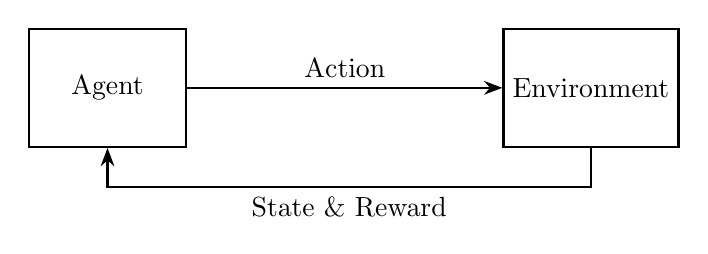
\begin{tikzpicture}[
			box/.style={draw, thick, rectangle, minimum width=2cm, minimum height=1.5cm},
			arrow/.style={thick, -Stealth}
		]

		% Draw the boxes
		\node[box] (agent) {Agent};
		\node[box, right=4cm of agent] (environment) {Environment};

		% Draw the arrows
		\draw[arrow] (agent.east) -- node[above] {Action} (environment.west);
		\draw[arrow] (environment.south) -- ++(0,-0.5) -| node[pos=0.25, below] {State \& Reward} (agent.south);

		\end{tikzpicture}
	\end{center}

	\newpage
	\section{Linear Regression}
	\label{sec:LinearRegression}

	\subsection{What is Regression?}
	\label{subsec:WhatIsRegression}

	\definition{Regression is a statistical modeling approach used to estimate the \highlightgreentext{relationship between a dependent variable and one or several independent variables that may contain errors}. The aim of regression is to identify the most suitable line or curve that represents the connection between the variables.}

	The fundamental concept of regression can be illustrated through the following steps: 
	\begin{enumerate}
		\item Consider a training set $S = \{(\mathbf{x}^{(l)}, \mathbf{y}^{(l)})\}_{l=1}^N$ which comprises $N$ pairs of inputs and corresponding outputs, with $\mathbf{x}^{(l)}$ representing the input and $\mathbf{y}^{(l)}$ denoting the output. 
		\item The input $\mathbf{x} = (x_1, x_2, \ldots, x_d)$ represents a vector in $d$ dimensions, with $d$ denoting the count of features or attributes. 
		\item \highlightbluetext{Regression Function $f(\cdot ; \mathbf{w})$} employs $S$ to ensure the predicted outcome $f(\mathbf{x}^{(l)} ; \mathbf{w})$ is as near as feasible to the true output $\mathbf{y}^{(l)}$ for every $l = 1, \ldots, N$, with $\mathbf{w}$ representing the parameter vector of the regression function. 
		\item When the output $\mathbf{y}$ consists of a multivariate vector, it represents a \highlightgreentext{multi-output regression} issue. For a univariate result, it constitutes a \highlightgreentext{single-output regression} issue. 
	\end{enumerate}

	\subsection{Linear Regression Function}
	\label{subsec:LinearRegressionFunction}
	If the regression function $f(\mathbf{x} ; \mathbf{w})$ is \highlightbluetext{linear}, it can be expressed as:
	\begin{equation}
	\label{eq:LinearRegressionFunction}
	\boxed{f(\mathbf{x} ; \mathbf{w}) = w_0 + w_1 x_1 + w_2 x_2 + \ldots + w_d x_d = \begin{bmatrix} w_0 & w_1 & w_2 & \ldots & w_d \end{bmatrix} \begin{bmatrix} 1 \\ x_1 \\ x_2 \\ \vdots \\ x_d \end{bmatrix} = \mathbf{w}^T \mathbf{\tilde{x}} = \mathbf{\tilde{x}}^T \mathbf{w}}
	\end{equation}
	
	\begin{itemize}
		\item Weight $w_0$ represents the \highlightbluetext{bias} term, which is a fixed value that acts as an adjustment for the regression function. 
		\item Learning problem involves identifying the optimal parameter vector $\mathbf{w} = (w_0, w_1, \ldots, w_d)$ that reduces the discrepancy between the predicted output $f(\mathbf{x}^{(l)} ; \mathbf{w})$ and the actual output $\mathbf{y}^{(l)}$ for every $l = 1, \ldots, N$.
	\end{itemize}

	\subsection{Squared Loss Function}
	\label{subsec:SquaredLossFunction}
	To determine the parameter vector $\mathbf{w}$ of the linear regression function $f(\mathbf{x}; \mathbf{w})$, it is essential to establish a loss function $L(\mathbf{w}; S)$ that measures the discrepancy between the predicted output and the true output. The loss function most frequently utilized for linear regression is the \highlightbluetext{squared loss function}, defined as:
	\begin{equation}
	\label{eq:SquaredLossFunction}
	\boxed{L(\mathbf{w}; S) = \sum_{l=1}^N \left( f(\mathbf{x}^{(l)}; \mathbf{w}) - \mathbf{y}^{(l)} \right)^2 = \sum_{l=1}^N \left( w_0 + w_1 x_1^{(l)} + w_2 x_2^{(l)} + \ldots + w_d x_d^{(l)} - \mathbf{y}^{(l)} \right)^2}
	\end{equation}

	The \highlightbluetext{mean squared error} (MSE) can be defined as the average of the squared loss function across all $N$ training samples:
	\begin{equation}
	\label{eq:MeanSquaredError}
	\boxed{\text{MSE}(\mathbf{w}; S) = \frac{1}{N} L(\mathbf{w}; S) = \frac{1}{N} \sum_{l=1}^N \left( f(\mathbf{x}^{(l)}; \mathbf{w}) - \mathbf{y}^{(l)} \right)^2}
	\end{equation}

	\newpage
	The squared loss function has two scenarios: $d = 1$ and $d > 1$, with $d$ representing the count of features in the input $\mathbf{x}$.

	\subsubsection{Special Case: Single-Output Regression ($d = 1$)}
	\label{subsubsec:SingleOutputRegression}
	Considering the squared loss function for single-output regression, the loss function can be represented as:
	\begin{equation}
	\label{eq:SingleOutputRegressionLossFunction}
	\boxed{L(w_0, w_1; S) = \sum_{l=1}^N \left( w_0 + w_1 x^{(l)} - y^{(l)} \right)^2}
	\end{equation}
	The distinctive optimal solution $\mathbf{w} = \begin{bmatrix} w_0 \\ w_1 \end{bmatrix}$ can be obtained by minimizing the loss function $L(w_0, w_1; S)$ through the least squares technique. 
	
	To find the optimal solution, one can calculate the partial derivatives of the loss function concerning $w_0$ and $w_1$, equate them to zero, and resolve the resulting equations:
	\begin{align*}
	\frac{\partial L}{\partial w_0} &= 2 \sum_{l=1}^N \left( w_0 + w_1 x^{(l)} - y^{(l)} \right) \cdot 1 = 0 \implies \sum_{l=1}^N \left( w_0 + w_1 x^{(l)}\right) = \sum_{l=1}^N y^{(l)} \implies Nw_0 + w_1 \sum_{l=1}^N x^{(l)} = \sum_{l=1}^N y^{(l)} \\
	\frac{\partial L}{\partial w_1} &= 2 \sum_{l=1}^N \left( w_0 + w_1 x^{(l)} - y^{(l)} \right) x^{(l)} = 0 \implies w_0 \sum_{l=1}^N x^{(l)} + w_1 \sum_{l=1}^N x^{(l)^2} = \sum_{l=1}^N y^{(l)} x^{(l)}
	\end{align*}
	We have a system of linear equations consisting of two equations and two unknown variables, which can be represented in matrix notation as:
	\begin{equation}
	\label{eq:SingleOutputRegressionMatrixForm}
	\boxed{\mathbf{Aw} = \begin{bmatrix} N & \sum_{l=1}^N x^{(l)} \\ \sum_{l=1}^N x^{(l)} & \sum_{l=1}^N x^{(l)^2} \end{bmatrix} \begin{bmatrix} w_0 \\ w_1 \end{bmatrix} = \begin{bmatrix} \sum_{l=1}^N y^{(l)} \\ \sum_{l=1}^N y^{(l)} x^{(l)} \end{bmatrix} = \mathbf{b}}
	\end{equation}
	Assuming the matrix $\mathbf{A}$ is invertible, the optimal solution can be found by multiplying both sides of the equation by $\mathbf{A}^{-1}$:
	\begin{equation}
	\label{eq:SingleOutputRegressionOptimalSolution}
	\boxed{\mathbf{w} = \mathbf{A}^{-1} \mathbf{b}}
	\end{equation}

	\subsubsection{General Case: Multi-Output Regression ($d > 1$)}
	\label{subsubsec:MultiOutputRegression}
	In multi-output regression, two methods can be used to identify the best solution. 
	
	The initial strategy is to utilize the \highlightbluetext{least squares method}. Initially, we represent the input and output sections of the $N$ examples as:
	\begin{align*}
		\mathbf{X} = \begin{bmatrix}
			1 & x_1^{(1)} & x_2^{(1)} & \ldots & x_d^{(1)} \\
			1 & x_1^{(2)} & x_2^{(2)} & \ldots & x_d^{(2)} \\
			\vdots & \vdots & \vdots & \ddots & \vdots \\
			1 & x_1^{(N)} & x_2^{(N)} & \ldots & x_d^{(N)}
		\end{bmatrix} \in \mathbb{R}^{N \times (d + 1)} \quad \text{and} \quad
		\mathbf{Y} = \begin{bmatrix}
			y_1^{(1)} \\
			y_2^{(1)} \\
			\vdots \\
			y_d^{(N)}
		\end{bmatrix} \in \mathbb{R}^{N \times d}
	\end{align*}
	We obtain a system of $d + 1$ linear equations involving $d + 1$ unknowns, which can be represented in matrix form as:
	\begin{equation}
	\label{eq:MultiOutputRegressionMatrixForm}
	\boxed{\mathbf{Aw} = (\mathbf{X}^T \mathbf{X}) \mathbf{w} = \mathbf{X}^T \mathbf{y} = \mathbf{b}}
	\end{equation}
	Assuming the matrix $\mathbf{A} = \mathbf{X}^T \mathbf{X}$ is invertible, one can determine the optimal solution by multiplying both sides of the equation by $\mathbf{A}^{-1}$:
	\begin{equation}
	\label{eq:MultiOutputRegressionOptimalSolution}
	\boxed{\mathbf{w} = \mathbf{A}^{-1} \mathbf{b} = (\mathbf{X}^T \mathbf{X})^{-1} \mathbf{X}^T \mathbf{y}}
	\end{equation}

	\newpage
	An alternative method is to differentiate using \highlightbluetext{Multivariable Calculus}. Initially, we can represent $\mathbf{Xw} - \mathbf{Y}$ as:
	\begin{align*}
		\mathbf{Xw} - \mathbf{Y} = \begin{bmatrix}
			1 & x_1^{(1)} & x_2^{(1)} & \ldots & x_d^{(1)} \\
			1 & x_1^{(2)} & x_2^{(2)} & \ldots & x_d^{(2)} \\
			\vdots & \vdots & \vdots & \ddots & \vdots \\
			1 & x_1^{(N)} & x_2^{(N)} & \ldots & x_d^{(N)} 
		\end{bmatrix} \begin{bmatrix} w_0 \\ w_1 \\ w_2 \\ \vdots \\ w_d \end{bmatrix} - \begin{bmatrix}
			y^{(1)} \\ y^{(2)} \\ \vdots \\ y^{(N)}
		\end{bmatrix} = \begin{bmatrix}
			w_0 + w_1 x_1^{(1)} + w_2 x_2^{(1)} + \ldots + w_d x_d^{(1)} - y^{(1)} \\
			w_0 + w_1 x_1^{(2)} + w_2 x_2^{(2)} + \ldots + w_d x_d^{(2)} - y^{(2)} \\
			\vdots \\
			w_0 + w_1 x_1^{(N)} + w_2 x_2^{(N)} + \ldots + w_d x_d^{(N)} - y^{(N)}
		\end{bmatrix}
	\end{align*}
	The squared loss function can be represented as the \highlightgreentext{squared L-2 norm of the vector} $\mathbf{Xw} - \mathbf{y}$:
	\begin{equation}
	\label{eq:MultiOutputRegressionSquaredLossFunction}
	\boxed{L(\mathbf{w}; S) = \left\| \mathbf{Xw} - \mathbf{y} \right\|^2}
	\end{equation}
	Then we can express the squared loss function as:
	\begin{align*}
		L(\mathbf{w}; S) = \left( \mathbf{Xw} - \mathbf{y} \right)^T \left( \mathbf{Xw} - \mathbf{y} \right) = \mathbf{w}^T \mathbf{X}^T \mathbf{X} \mathbf{w} - 2 \mathbf{y}^T \mathbf{X} \mathbf{w} + \mathbf{y}^T \mathbf{y}
	\end{align*}
	To reduce the squared loss function, we can calculate the gradient of $L(\mathbf{w}; S)$ concerning $\mathbf{w}$ and equate it to zero:
	\begin{align*}
		\nabla_{\mathbf{w}} L(\mathbf{w}; S) = 2 \mathbf{X}^T \mathbf{X} \mathbf{w} - 2 \mathbf{X}^T \mathbf{y} = 0
		&\implies \mathbf{X}^T \mathbf{X} \mathbf{w} = \mathbf{X}^T \mathbf{y} \\
		&\implies \mathbf{w} = \left( \mathbf{X}^T \mathbf{X} \right)^{-1} \mathbf{X}^T \mathbf{y}
	\end{align*}

	To find the optimal solution $\mathbf{w}$, we must compute the inverse of the matrix $\mathbf{X}^T \mathbf{X} \in \mathbb{R}^{(d + 1) \times (d + 1)}$. We can apply the \highlightbluetext{LeGall algorithm}, recognized as the quickest identified method for matrix multiplication, exhibiting a \highlightgreentext{time complexity of $O(n^{2.3728596})$} for an $n \times n$ matrix, in contrast to the straightforward $O(n^3)$ approach used in Cholesky decomposition, LU decomposition, or Gaussian elimination.

	\subsection{Nonlinear Extension of Linear Regression}
	\label{subsec:NonlinearExtensionOfLinearRegression}
	Nonlinear regression functions are crucial because more complex issues cannot be addressed by linear regression. To tackle this, we can modify the linear regression function $f(\mathbf{x}; \mathbf{w})$ into a nonlinear format by adding nonlinear transformations of the input features. Three distinct methods exist for nonlinear expansions to accomplish this:
	\begin{enumerate}
		\item \highlightbluetext{Feature Engineering}: Intentionally generate additional input dimensions (nonlinearly related to the original input) and utilize linear regression on the newly created input dimensions. For instance, if the original input is $\mathbf{x} = (x_1, x_2)$, we can generate additional features like $x_1^2$, $x_2^2$, and $x_1 x_2$ to create an updated input $\mathbf{\tilde{x}} = (1, x_1, x_2, x_1^2, x_2^2, x_1 x_2)$. 

		The key benefit is that linear regression remains applicable, and the weights in the model are \highlightgreentext{highly interpretable} (the greater the weight's magnitude, the more significant the feature). The primary drawback is that it necessitates domain expertise to develop new features and can be costly in terms of computation if the feature count is high.
		\begin{center}
			\scalebox{0.8}{
			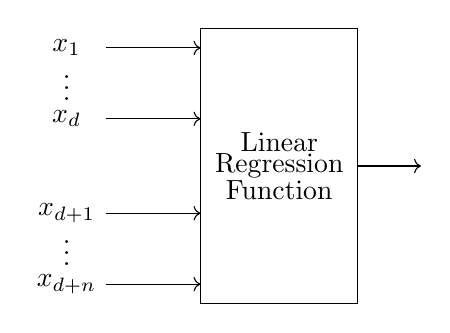
\begin{tikzpicture}
				\node at (0, 0) {$x_1$};
				\node at (0, -0.4) {$\vdots$};
				\node at (0, -0.9) {$x_d$};
				\node at (0, -2.1) {$x_{d +1}$};
				\node at (0, -2.5) {$\vdots$};
				\node at (0, -3.0) {$x_{d + n}$};
				\draw[->] (0.5, 0) -- (1.7, 0);
				\draw[->] (0.5, -0.9) -- (1.7, -0.9);
				\draw[->] (0.5, -2.1) -- (1.7, -2.1);
				\draw[->] (0.5, -3.0) -- (1.7, -3.0);

				\draw (1.7, 0.25) rectangle (3.7, -3.25);
				\node at (2.7, -1.2) {Linear};
				\node at (2.7, -1.5) {Regression};
				\node at (2.7, -1.8) {Function};

				\draw[->] (3.7, -1.5) -- (4.5, -1.5);
			\end{tikzpicture}}
		\end{center}

		\newpage
		\item \highlightbluetext{Explicit Mapping}: Apply an explicitly defined \highlightgreentext{nonlinear regression function} $f(\mathbf{x}; \mathbf{w})$ that is nonlinear in the input $\mathbf{x}$, such as polynomial regression, radial basis function (RBF) regression, or neural networks. The model learns the parameters $\mathbf{w}$ of the nonlinear function directly from the training data.
		
		\begin{center}
			\scalebox{0.8}{
			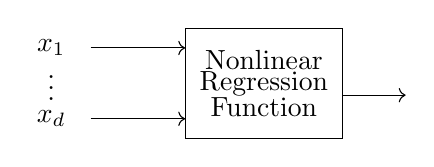
\begin{tikzpicture}
				\node at (0, 0) {$x_1$};
				\node at (0, -0.4) {$\vdots$};
				\node at (0, -0.9) {$x_d$};
				\draw[->] (0.5, 0) -- (1.7, 0);
				\draw[->] (0.5, -0.9) -- (1.7, -0.9);

				\draw (1.7, 0.25) rectangle (3.7, -1.15);
				\node at (2.7, -0.15) {Nonlinear};
				\node at (2.7, -0.45) {Regression};
				\node at (2.7, -0.75) {Function};

				\draw[->] (3.7, -0.6) -- (4.5, -0.6);
			\end{tikzpicture}}
		\end{center}

		\item \highlightbluetext{Implicit Mapping}: Implement an \highlightgreentext{implicitly defined nonlinear transformation} on the original input, followed by utilizing a linear regression function on the modified input. This method employs kernel techniques or neural networks with latent layers to automatically acquire valuable feature representations without their explicit specification. For instance, kernel techniques such as Support Vector Machines (SVM) implicitly transform the input into a higher-dimensional space via kernel functions.

		\begin{center}
			\scalebox{0.8}{
			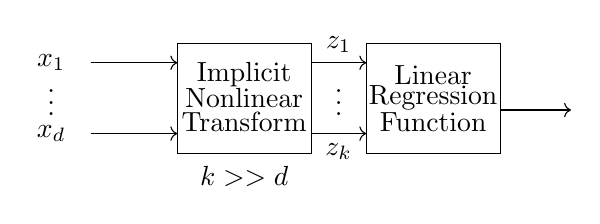
\begin{tikzpicture}
				\node at (0, 0) {$x_1$};
				\node at (0, -0.4) {$\vdots$};
				\node at (0, -0.9) {$x_d$};
				\draw[->] (0.5, 0) -- (1.6, 0);
				\draw[->] (0.5, -0.9) -- (1.6, -0.9);

				\draw (1.6, 0.25) rectangle (3.3, -1.15);
				\node at (2.45, -1.45) {$k >> d$};
				\node at (2.45, -0.15) {Implicit};
				\node at (2.45, -0.45) {Nonlinear};
				\node at (2.45, -0.75) {Transform};

				\draw[->] (3.3, 0) -- (4.0, 0) node [midway, above] {$z_1$};
				\node at (3.65, -0.4) {$\vdots$};
				\draw[->] (3.3, -0.9) -- (4.0, -0.9) node [midway, below] {$z_k$};

				\draw (4.0, 0.25) rectangle (5.7, -1.15);
				\node at (4.85, -0.15) {Linear};
				\node at (4.85, -0.45) {Regression};
				\node at (4.85, -0.75) {Function};

				\draw[->] (5.7, -0.6) -- (6.6, -0.6);
			\end{tikzpicture}}
		\end{center}
	\end{enumerate}

	\subsection{Polynomial Regression}
	\label{subsec:PolynomialRegression}
	Polynomial Regression introduces higher-order polynomial terms as the additional input features in the linear regression function. The polynomial regression function can be expressed as:
	\begin{equation}
		\boxed{f(\mathbf{x}; \mathbf{w}) = w_0 + w_1 x + \ldots + w_m x^m = \begin{bmatrix} w_0 & w_1 & \ldots & w_m \end{bmatrix} \begin{bmatrix} 1 \\ x \\ \vdots \\ x^m \end{bmatrix} = \mathbf{w}^T \mathbf{\tilde{x}} = \mathbf{\tilde{x}}^T \mathbf{w}}
	\end{equation}
	\begin{itemize}
		\item The parameter vector $\mathbf{w} = (w_0, w_1, \ldots, w_m)$ consists of $m + 1$ parameters, where $m$ is the degree of the polynomial. 
		\item The input $\mathbf{\tilde{x}} = (1, x, x^2, \ldots, x^m)$ represents the polynomial features derived from the original input $x$.
	\end{itemize}
	Although $f(\mathbf{x}; \mathbf{w})$ is nonlinear with respect to the input $x$, it stays linear concerning the parameters $\mathbf{w}$. Consequently, we can utilize the same least squares technique to determine the ideal parameter vector $\mathbf{w}$ by minimizing the squared loss function.

	Additionally, we can employ \highlightgreentext{broader transformations} of the initial input dimensions to develop polynomial features. For example, feature engineering can specify the features tailored to the application that are used on the input data, including interaction terms or transformations specific to the domain. Using body weight and body height as an illustration, the body mass index (BMI) will be the supplementary characteristic specified. The least squares method for linear regression remains applicable to determine the optimal parameter vector $\mathbf{w}$ for acquiring the \highlightgreentext{closed form solution}.

	\subsection{Regularization}
	\label{subsec:Regularization}
	Regularization is a technique that alters the original loss function by incorporating one or more penalty terms known as \highlightbluetext{regularizers} that discourage large parameter values to avoid overfitting due to excessively high parameter magnitudes.

	\newpage

	\highlightbluetext{Overfitting} arises when the \highlightgreentext{training dataset $S = \{(\mathbf{x}^{(l)}, \mathbf{y}^{(l)})\}_{l=1}^N$ is limited in size relative to the number of parameters in the linear regression model $f(\mathbf{x}; \mathbf{w})$}. In this scenario, the model could discover significant values in certain parameters, as an expanded search space enables the model to align more closely with the training data, which may result in inadequate generalization on new data.

	Regularization helps tackle this issue by constraining the magnitude of the parameters, promoting simpler models that are less likely to overfit the training data. The \highlightbluetext{loss function with regularization} employing \highlightbluetext{$L_2$ regularization / Tikhonov regularization} can be represented as:
	\begin{equation}
	\label{eq:RegularizedLossFunction}
	\boxed{L_{\lambda}(\mathbf{w}; S) = L(\mathbf{w}; S) + \lambda \|\mathbf{w}\|^2 = \|\mathbf{Xw} - \mathbf{y}\|^2 + \lambda \|\mathbf{w}\|^2 = \mathbf{w}^T \mathbf{X}^T \mathbf{X} \mathbf{w} - 2 \mathbf{y}^T \mathbf{X} \mathbf{w} + \mathbf{y}^T \mathbf{y} + \lambda \mathbf{w}^T \mathbf{w}}
	\end{equation}
	\begin{itemize}
		\item The parameter $\lambda > 0$ serves as a \highlightbluetext{regularization hyperparameter} that regulates the intensity of the regularization, established during the validation phase. \\
		A greater $\lambda$ produces more intense regularization, whereas a lesser $\lambda$ causes weaker regularization.
		\item The notation $\|\mathbf{w}\|^2$ signifies the squared L2 norm of the parameter vector $\mathbf{w}$, imposing a penalty on large parameter values.
	\end{itemize}
	In practice, the bias $w_0$ is frequently left out of the regularization term since it merely acts as an \highlightgreentext{offset} and does not add to the model's complexity. The loss function with regularization can be optimized through techniques like gradient descent or by utilizing \highlightgreentext{closed-form solutions}.

	To find the closed-form solution with $L_2$ regularization, we can differentiate the loss function $L_{\lambda}(\mathbf{w}; S)$ with respect to $\mathbf{w}$ and set it to zero:
	\begin{align*}
		2 \mathbf{X}^T \mathbf{X} \mathbf{w} - 2 \mathbf{X}^T \mathbf{y} + 2 \lambda \mathbf{w} = 0 \implies (\mathbf{X}^T \mathbf{X} + \lambda \mathbf{I}) \mathbf{w} = \mathbf{X}^T \mathbf{y} \quad \text{where } \mathbf{I} \text{ is the identity matrix}
	\end{align*}
	The closed-form solution for the least squares estimate of the parameter vector $\mathbf{w}$ with $L_2$ regularization can be defined as:
	\begin{equation}
	\label{eq:RegularizedClosedFormSolution}
	\boxed{\mathbf{w} = (\mathbf{X}^T \mathbf{X} + \lambda \mathbf{I})^{-1} \mathbf{X}^T \mathbf{y}} \quad \text{where } \mathbf{X}^T \mathbf{X} + \lambda \mathbf{I} \text{ is invertible for } \lambda > 0
	\end{equation}
	This regularized method is referred to as \highlightbluetext{Ridge Regression}. It minimizes overfitting and enhances the model's ability to generalize to new data by imposing penalties on large parameter values. Crucially, when the regularization parameter $\lambda$ is equal to zero, ridge Regression reduces to standard linear regression, since no penalty is enforced.

	\subsubsection{Choice of Regularization Parameter $\lambda$}
	\label{subsubsec:ChoiceOfRegularizationParameter}
	The regularization coefficient $\lambda$ is an essential hyperparameter that dictates the intensity of the regularization imposed on the model. The selection of $\lambda$ can greatly influence the performance of the model and is usually established via a validation process. A frequent method for determining the best value of $\lambda$ is to employ \highlightbluetext{cross-validation}.

	Cross-validation involves \highlightgreentext{splitting the training dataset into multiple subsets (folds) and training the model on one subset} while evaluating it on the remaining data. Subsequently, the trained model is \highlightgreentext{evaluated on a separate validation set} to resemble the test set. The procedure is carried out for different $\lambda$ values, and the model's effectiveness is assessed utilizing a specific metric (e.g., mean squared error, accuracy). The best performance on the validation set is achieved by choosing the optimal regularization parameter as the value of $\lambda$ with the smallest validation error.

	\newpage
	The standard training and validation error curves for various $\lambda$ values are illustrated below. 
	\begin{center}
		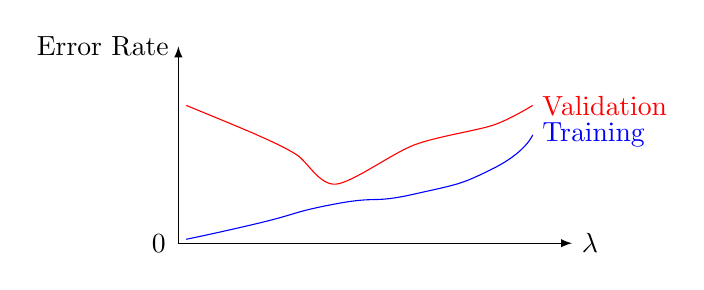
\begin{tikzpicture}[scale= 0.05]
			\draw [-latex](0, 0) -- (100, 0) node[right]{$\lambda$};
			\draw [-latex](0, 0) -- (0, 50) node[left]{Error Rate};
			\node (0, 0) at (-5, 0) {0};
			% Halved y-coordinates for both curves
			\draw [red] plot [smooth, tension=0.5] coordinates {(2, 35) (20, 27.5) (30, 22.5) (40, 15) (60, 25) (80, 30) (90, 35)} node[right]{Validation};
			\draw [blue] plot [smooth, tension=1] coordinates { (2, 1) (20, 5) (40, 10) (60, 12.5) (80, 19) (90, 27.5)} node[right]{Training};
		\end{tikzpicture}
	\end{center}
	The training error usually rises with an increase in $\lambda$, whereas the validation error first drops and then rises, suggesting that \highlightgreentext{a low $\lambda$ causes overfitting whereas a high $\lambda$ leads to underfitting}.

	\subsubsection{Other Regularization Techniques}
	\label{subsubsec:OtherRegularizationTechniques}
	In addition to $L_2$ regularization, other approaches can also be used to prevent overfitting in machine learning models. A general framework for these methods is provided by the $L_p$ norm, which generalizes both the $L_1$ and $L_2$ norms. By varying the value of $p$, a family of regularization strategies can be defined:
	\begin{equation}
		\boxed{\|\mathbf{v}\|_p = \left( \sum_{i=1}^{n} |v_i|^p \right)^{1/p} \quad \text{for } p \geq 1}
	\end{equation}
	Among these, \highlightbluetext{$L_1$ regularization}, known as \highlightbluetext{LASSO (Least Absolute Shrinkage and Selection Operator)}, is especially popular. LASSO adds a penalty term based on the $L_1$ norm of the parameter vector $\mathbf{w}$ to the loss function, which encourages sparsity by driving many coefficients to exactly zero:
	\begin{equation}
	\label{eq:LassoLossFunction}
		\boxed{L_{\lambda}(\mathbf{w}; S) = L(\mathbf{w}; S) + \lambda \|\mathbf{w}\|_1 = \|\mathbf{Xw} - \mathbf{y}\|^2 + \lambda \sum_{i=0}^{d} |w_i|}
	\end{equation}
	While $L_1$ regularization leads to a convex optimization problem, it does not admit a closed-form solution. Instead, iterative optimization algorithms such as coordinate descent or subgradient descent are typically used to find the optimal parameter vector $\mathbf{w}$.

	\subsection{Common Performance Metrics for Linear Regression}
	\label{subsec:CommonPerformanceMetricsForLinearRegression}
	To evaluate the performance of linear regression models, several metrics are commonly used. These metrics help assess how well the model predicts the target variable and can guide improvements in model design. Two of the most widely used metrics are \highlightbluetext{Mean Squared Error (MSE)} and \highlightbluetext{R-squared Scores}.

	\subsubsection{Mean Squared Error (MSE)}
	\label{subsubsec:MeanSquaredError}
	Once a regression model has been trained, it is crucial to quantitatively evaluate how accurately the model's predictions align with the real target values. A commonly utilized metric for this aim is the \highlightbluetext{Mean Squared Error (MSE)}. MSE computes the \highlightgreentext{mean of the squared deviations between the predicted values and the actual target values for all samples}. It is described as:
	\begin{equation}
	\label{eq:MeanSquaredErrorDefinition}
		\boxed{\text{MSE} = \frac{1}{N} \sum_{l = 1}^{N} \left( f(\mathbf{x}^{(l)}; \mathbf{w}) - \mathbf{y}^{(l)} \right)^2 = \frac{1}{N} L(\mathbf{w}; S)}
	\end{equation}
	\begin{itemize}
		\item $N$ is the total number of samples in the dataset, $f(\mathbf{x}^{(l)}; \mathbf{w})$ is the predicted value for the $l$-th sample, and $\mathbf{y}^{(l)}$ is the corresponding true value.
	\end{itemize}
	MSE can be calculated on the training set, validation set, or test set to assess model performance and generalization.

	Nonetheless, since MSE is represented in the squared units of the target variable, interpreting it directly can be challenging. To tackle this, the \highlightbluetext{Root Mean Squared Error (RMSE)} is commonly employed, as it calculates the square root of the MSE to revert the error to the initial scale of the target variable:
	\begin{equation}
	\label{eq:RootMeanSquaredErrorDefinition}
		\boxed{\text{RMSE} = \sqrt{\text{MSE}} = \sqrt{\frac{1}{N} \sum_{l = 1}^{N} \left( f(\mathbf{x}^{(l)}; \mathbf{w}) - \mathbf{y}^{(l)} \right)^2}}
	\end{equation}
	Consequently, RMSE is easier to understand and gives a clear indication of the usual size of prediction errors in the same units as the target variable.

	\subsubsection{R-squared ($R^2$) Score}
	\label{subsubsec:RSquaredScore}
	Though MSE and RMSE offer an absolute assessment of prediction error, having a relative metric that shows how effectively the model accounts for the variability in the target variable against a basic baseline is often beneficial. The \highlightbluetext{R-squared ($R^2$) value}, often referred to as the \highlightbluetext{coefficient of determination}, fulfills this role.

	$R^2$ measures the fraction of the overall variability in the target variable that the model's predictions explain. It is characterized as:
	\begin{equation}
	\label{eq:RSquaredScoreDefinition}
		\boxed{R^2 = 1 - \frac{\sum_{l = 1}^{N} \left( f(\mathbf{x}^{(l)}; \mathbf{w}) - \mathbf{y}^{(l)} \right)^2}{\sum_{l = 1}^{N} \left( \mathbf{y}^{(l)} - \bar{\mathbf{y}} \right)^2} = 1 - \frac{\text{MSE}}{\text{VAR}(\mathbf{y})}} \quad \text{where } \bar{\mathbf{y}} = \frac{1}{N} \sum_{l = 1}^{N} \mathbf{y}^{(l)} \text{ is the mean of the target variable}
	\end{equation}
	\begin{itemize}
		\item The numerator is the residual sum of squares (RSS), indicating the variance that remains unexplained (the discrepancy between predicted and actual values).
		\item The denominator is the total sum of squares (TSS), which indicates the overall variance in the target variable concerning its average.
	\end{itemize}
	$R^2$ varies between 0 and 1, with \highlightgreentext{1 indicating that the model completely accounts for all variability} in the target variable, and \highlightgreentext{0 signifying no explanation} at all (similar to predicting the average consistently). Negative $R^2$ values may arise when the model is less effective than merely predicting the average, signifying inadequate model fit.

	\newpage
	\section{Logistic Regression}
	\label{sec:LogisticRegression}

	\subsection{What is Logistic Regression?}
	\label{subsec:WhatIsLogisticRegression}

\end{document}